%
% File naaclhlt2010.tex
%
% Contact: nasmith@cs.cmu.edu

\documentclass[11pt,letterpaper]{article}
\usepackage{naaclhlt2010}
\usepackage{times}
\usepackage{latexsym}
\usepackage{verbatim}
\usepackage{graphicx}
\usepackage{rotating}
\usepackage[table]{xcolor}
%  Linguistics article environments in LaTeX
%  R.L.H. - EUROTRA PROJECT, Dept. Lang & Ling, University of Essex
%  Mar 16 90
%	Revised Aug 90
%
%
%  Input this file into your source file by putting the LaTeX command
%  `` \input <thisfilename> '' on its first line.
%
% `%' starts a comment !

%%	*********** Macro Definitions **************
%%
% LINGUISTIC ITEM ENVIRONMENT
% Linguistic items (examples, diagrams, trees etc) are normally
% numbered consecutively throughout a linguistic article.

\newcounter{licntr}			% linguistic item counter

% Two commands required in the defintion of a linguistic item
\newcommand{\stepli}{\refstepcounter{licntr}}	% increment
					  	% li counter
\newcommand{\lival}{\thelicntr}			% return value
						% of li
						% counter
%% Now we define the ``linguistic item'' environment for cases where
%% there is just one \item to be displayed e.g. a single sentence
%% First, define the outer environment (which handles the numbering)
\newenvironment{liout}{\small
		\stepli			% step li counter
		\samepage			% prevent page break
		\begin{list}{		% begin definition
			(\lival)\hfill}{} 	% left adjust number
			\samepage
			\item 			% dummy item
		}{ \end{list}}

\newenvironment{liexc}{\small
		\samepage			% prevent page break
		\begin{list}{		% begin definition
			(27)\hfill}{} 	% left adjust number
			\samepage
			\item 			% dummy item
		}{ \end{list}}

%% Now embed a new list in the outer list - to typographical match the
%% ``lis'' environment (where we have alpha-indexed items)
\newenvironment{li}{\small
		\begin{liout} 			% begin outer list
		\begin{list}{\samepage \noindent}{} 	% begin inner
						% list,  prevent page break 
		\item}{				% item
		\end{list} 
		\end{liout}}

\newenvironment{liexcp}{\small
		\begin{liexc} 			% begin outer list
		\begin{list}{\samepage \noindent}{} 	% begin inner
						% list,  prevent page break 
		\item}{				% item
		\end{list} 
		\end{liexc}}



%% Special version of li which does NOT indent material - puts number
%% on line by itself and then (unindented) material below
\newenvironment{li*}{\small
	\stepli
	\samepage				% prevent page break
	\begin{trivlist} \item[] (\lival) \end{trivlist}
	\begin{trivlist} 
	{\samepage \item[]}
	}{\end{trivlist}}					% space
				

% LINGUISTIC ITEMS ENVIRONMENT
% Define a counter for alphabetically indexed items
\newcounter{alphcntr}		% will be reset in each new lis environment

% Define an environment (called ``lis'' = linguistic items) for a
% series of alpha-indexed linguistic items e.g. 
%	(1) a.
%	    b.    etc.
\newenvironment{lis}{\small
		\begin{liout} 				% begin outer list
			\begin{list}{			% begin inner
							% list
				\samepage		% prevent pg breaks
				\alph{alphcntr}.\hfill 	%left-align letter
					}{
				\usecounter{alphcntr}}}{
		\end{list} \end{liout}}

% LINGUISTIC PRINCIPLE COMMAND - \princ
\newtheorem{prin}{Principle}
%%\newtheorem{ax}{Axiom}
%%\newtheorem{fig}{Figure}
\newtheorem{assum}{Assumption}
\newtheorem{defn}{Definition}
% Define any more you want here.....

% Now define a command with two arguments to handle linguistic
% principles.  The command - ``princ'' takes two arguments: the
% first is the name associated with a \newtheorem (e.g. ``prin'') and
% the second  is the text of that principle. (We use a command here
% rather than an  environment due to technical limitations of LaTeX environment
% parameter handling.)
\newcommand{\princ}[2]{\begin{liout} 
			\begin{#1} 
				{#2}
			\end{#1}
			\end{liout}}
			
			
% MACROS FOR PRODUCING LABELLED/UNLABELLED BRACKETS
\newcommand{\lb}{\mbox{$ [ $}}			% unlabelled right
						% bracket 

\newcommand{\rb}{\mbox{$ ] $}}			% unlabelled right
						% bracket 

\newcommand{\llb}[1]{\mbox{$ [_{#1} $}}		% labelled left
						% bracket

\newcommand{\lrb}[1]{\mbox{$ ]_{#1} $}}   	% labelled right
					      	% bracket

% MACROS FOR HANDLING LISTS, SHORTCUTS etc - A.W., 13/1/95
\newcommand{\bi}{\begin{itemize}}		 
\newcommand{\ei}{\end{itemize}}		 

\newcommand{\be}{\begin{enumerate}}		 
\newcommand{\ee}{\end{enumerate}}

\newcommand{\bc}{\begin{center}}		
\newcommand{\ec}{\end{center}}		

\newcommand{ \heading }[1]{ \begin{center}
			   {\bf {#1}}
			    \end{center}}

% MACROS FOR STANDARD LINGUISTIC SYMBOLS (can be used in text mode)
\newcommand{\tarr}{\mbox{$ \Longrightarrow $}}	% ==> i.e
						% translation arrow

\newcommand{\rarr}{\mbox{$ \longrightarrow $}}	% --> i.e.
						% rule arrow

\newcommand{\llr}{\mbox{$ \longleftrightarrow $}}	% <--> i.e.
						% rule arrow

\newcommand{\up}{\mbox{$ \uparrow $}}	% uparrow for text/maths
						% environment

\newcommand{\down}{\mbox{$ \downarrow $}}	% downarrow for
					    	% text/maths environment

%% \newcommand{\th}{\mbox{$ \theta $}}		% theta
\newcommand{\al}{\mbox{$ \alpha $}}		% alpha

% MACROS FOR ASTERISKING LINGUISTIC DATA
% (ensures data strings are neatly aligned e.g
%	Green ideas sleep furiously
%      *Green ideas furious sleep

\newlength{\astspace}				% initialise length command

\settowidth{\astspace}{\mbox{$\ast$}}		% set length command
						% to width of an asterisk

\newcommand{\un}{\mbox{$\ast$}}			% unacceptable string (*)

\newcommand{\qu}{?}				% questionable string

\newcommand{\ac}{\hspace*{\astspace}}		% acceptable string
						% (inserts *-width
						% space at start of
						% string)

%% ATTRIBUTE-VALUE ARRAY ENVIRONMENT		
%% Now we define some specialised linguistic items, starting with an
%% attribute value array
\newcommand{\attrib}[1]{{\rm \bf {#1}}}		% define the
						% attributes of an
						% attribute

\newcommand{\atomval}[1]{{\rm {#1}}}		% define attribute of
						% an atomic value

\newcommand{\sematomval}[1]{{\mit {#1}}}	% define attribute of 
						% semantic atomic values

% Att-Val array environment.  
% Must occur inside maths environment
\newenvironment{av}{\left[ \begin{array}{ll}}{\end{array} \right]}

%% Labelled Att-Val array environment
\newenvironment{lav}[1]{ \left[_{#1} \begin{array}{ll}}{\end{array} \right]}


%% TREE ENVIRONMENT - \begin{tree}{}......\end{tree}
% Trees produced by specialised tabular environment which takes an
% argument corresponding to the width of the tree - a string in c*
% e.g. cccc  for a tree 4 nodes wide. Lines between nodes must be   
% drawn by hand. 
\newenvironment{tree}[1]{		
	\begin{large}				% nodes in large typeface
	\renewcommand{\arraystretch}{4}		% set interrow space
						% to 4 (LaTeX default
						% is 1.  Change this
						% value to increase
						% depth of subtrees.
						% Range 3-6  approx

	\begin{tabular}{{#1}} 			% begin tree with 
						% argument-specified width
	\addtolength{\tabcolsep}{\tabcolsep}	% Double normal table
					    	% column separation. 
	}{				

	\addtolength{\tabcolsep}{-0.5\tabcolsep}	% Restore normal table
					     	% column separation
	\end{tabular}				% end of tree description

	\renewcommand{\arraystretch}{1}		% Restore default
						% array row separation
	\end{large} }				% Back to normal size

%% Commands for drawing boxes around lists, from Arnold et al '94.

\newcommand{\dougswideboxfigure}[3]{	
\begin{figure}[hbtp]
\begin{center}
\begin{tabular}{|p{134mm}|}\hline
%{|@{\hspace{3em}}l@{\hspace{3em}}|}\hline
\\
\multicolumn{1}{|c|}{\bf #2}\\
% only one extra line here is better:\\
\begin{center}
\begin{minipage}[t]{110mm}
#3
\end{minipage}
\end{center}
\\
\hline
\end{tabular}
\end{center}
\label{#1}
\end{figure}
}



\newcounter{figcntr}			% figiom counter

% Two commands required in the defintion of an figiom
\newcommand{\stepfig}{\refstepcounter{figcntr}}	% increment
					  	% fig counter
\newcommand{\figval}{\thefigcntr}		% return value
						% of fig
						% counter

%% Now we define the ``linguistic item'' environment for cases where
%% there is just one \item to be displayed e.g. a single sentence
%% First, define the outer environment (which handles the numbering)
\newenvironment{figout}{
		\stepfig			% step fig counter
		\begin{list}{		% begin definition
			(\figval)\hfill}{} 	% left adjust number
			\item 			% dummy item
		}{ \end{list}}

%% Now embed a new list in the outer list - to typographical match the
%% ``lis'' environment (where we have alpha-indexed items)
\newenvironment{fig}{
		\samepage			% prevent page break
		\begin{figout} 			% begin outer list
		\begin{list}{}{} 		% begin inner list
		\item}{				% item
		\end{list} 
		\end{figout}}

\renewcommand{\thefigcntr}{\Alph{figcntr}}

\newcounter{axcntr}			% axiom counter

% Two commands required in the defintion of an axiom
\newcommand{\stepax}{\refstepcounter{axcntr}}	% increment
					  	% ax counter
\newcommand{\axval}{\theaxcntr}		% return value
						% of ax
						% counter

%% Now we define the ``linguistic item'' environment for cases where
%% there is just one \item to be displayed e.g. a single sentence
%% First, define the outer environment (which handles the numbering)
\newenvironment{axout}{
		\stepax			% step ax counter
		\begin{list}{		% begin definition
			(\axval)\hfill}{} 	% left adjust number
			\item 			% dummy item
		}{ \end{list}}

%% Now embed a new list in the outer list - to typographical match the
%% ``lis'' environment (where we have alpha-indexed items)
\newenvironment{ax}{
		\samepage			% prevent page break
		\begin{axout} 			% begin outer list
		\begin{list}{\noindent}{} 		% begin inner list
		\item}{				% item
		\end{list} 
		\end{axout}}

\renewcommand{\theaxcntr}{\Roman{axcntr}}

%EMBEDDED AXIOMS e.g.
%	(1) a.
%	    b.    etc.

\newcounter{alphacntr}		% will be reset in each new ax environment

\newenvironment{axs}{
		\begin{axout} 				% begin outer list
			\begin{list}{			% begin inner
							% list
				\samepage		% prevent pg breaks
				\alph{alphacntr}.\hfill %left-align letter
					}{
				\usecounter{alphacntr}}}{
		\end{list} \end{axout}}


\newcommand{\s}{\mbox{$ \sectionsymbol $}}      
\let\sectionsymbol=\S
\def\S{{}\;{}}


%%\usepackage{colortbl}
\setlength\titlebox{6.5cm}    % Expanding the titlebox

\title{Evaluating Non-Expert Annotations on Mechanical Turk for Opinion Mining on Spanish Data}

\author{\\
  \\
  \\
  \\
  }

\date{}

\begin{document}
\maketitle
\begin{abstract}
  One of the major bottlenecks in the development of data-driven AI Systems is the lack of reliable human annotations. The recent advent of several crowdsourcing platforms such as Amazon's Mechanical Turk, allowing requesters the access to affordable and rapid results of a global workforce, greatly facilitates the creation of massive training sets. Most of the available studies on the effectiveness of crowdsourcing report on English data. We use Mechanical Turk annotations to train an Opinion Mining System to classify Spanish consumer comments. We design three different Human Intelligence Task (HIT) strategies and show high inter-annotator agreement between non-experts and expert annotators. We evaluate the advantages/drawbacks of each HIT design and report \texttt{<results of the classifier>}.
\end{abstract}

\section{Introduction}
\label{sect:intro}
\texttt{<Intro.>}
\texttt{<Some possible citations for remainder paper.>}
In~\cite{snow_cheap_2008}, it is shown that $\ldots$ \\
In~\cite{sheng_get_2008}, it is shown that $\ldots$ \\
In~\cite{kittur_crowdsourcing_2008}, it is shown that $\ldots$ \\
In~\cite{su_internet-scale_2007}, it is shown that $\ldots$ \\

\section{Task Outline and Goals}
\label{sect:outline}

We compare different HIT design strategies by evaluating the usefulness of resulting Mechanical Turk (AMT) annotations to train an Opinion Mining System on Spanish consumer data. More specifically, we address the following research questions:\\
 \indent (i) Annotation quality: how do the different AMT annotations compare to expert annotations? We compare the inter-annotator agreement in expert annotations with the inter-annotator agreement in the different AMT annotations.\\
 \indent (ii) Annotation applicability: how does the performance of an Opinion Mining classifier vary after training on different (sub)sets of AMT and expert annotations? Given a simple classification technique, we evaluate the system performance by using AMT annotations, expert annotations and the combination of both as training data. The idea is not to evaluate the classification technique \textit{per se}, but to measure the influence of the training material.\\
 \indent (iii) Return on Investment (ROI): how does the use of AMT annotations compare economically against the use of expert annotations? AMT offers the possibility of obtaining inexpensive annotations the quality of which tends to be worse than expert annotations \texttt{<include ref>}. We show that, for the task at hand, the ROI is positive.\\
 \indent (iv) Language barriers: \texttt{x\%} of all AMT tasks are designed for English speakers \texttt{<include ref>}. How easy is it to get reliable AMT results for Spanish? 

\section{HIT Design}
\label{sect:design}

We selected a dataset of 1000 sentences containing user opinions on cars from the automotive section of \texttt{www.ciao.es} (Spanish). This website was chosen because it contains a large and varied pool of Spanish customer comments suitable to train an Opinion Mining System and because opinions include simultaneously global numeric and specific ratings over particular attributes of the subject matter. Section \ref{datasets} contains more detailed information about the selection of the dataset. An example of a sentence from the data set can be found in (\ref{ex}):

\begin{li}
  \label{ex}
  `No te lo pienses m\'{a}s, c\'{o}mpratelo!'\\
  ($=$ `Don't think twice, buy it!')
\end{li}

\begin{figure}
  \begin{center}
    \fbox{
    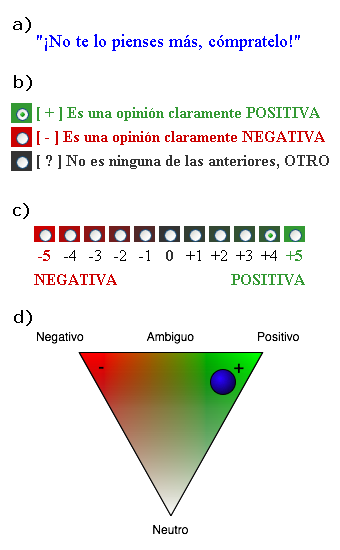
\includegraphics[scale=0.6]
	{pics/Reshots_All.png}}
	\caption{An example sentence (a) and the three HIT designs used in the experiments: (b) HIT1: a simple categorization scheme, (c) HIT2: a graded categorization scheme, and (d) HIT3: a continuous triangular categorization scheme containing both a horizontal positive-negative axis and a vertical subjective-objective axis.}
	\label{hits}
  \end{center}
\end{figure}

The sentences in the dataset were presented to the AMT workers in three different HIT designs. HIT1 is a simple categorization scheme in which workers are asked to classify each sentence as being either \textit{positive}, \textit{negative} or \textit{neutral}, as is shown in Figure \ref{hits}, section b. HIT2 is a graded categorization template in which workers had to assign a score between -5 (negative) and +5 (positive) to each example sentence, as is shown in Figure \ref{hits}, section c. Finally, HIT3 is a continuous triangular categorization template that allows workers to use both a horizontal positive-negative axis and a vertical subjective-objective axis by placing the example sentence anywhere inside the triangle. The subjective-objective axis expresses the degree to which the sentence contains opinionated content and was earlier used by \cite{sentiwordnet:06}. For example, the sentence \textit{`I think this is a wonderful car'} clearly marks an opinion and should be positioned towards the subjective end, while the sentence \textit{`The car has six cilinders'} should be located towards the objective end. Figure \ref{hits}, section d contains an example of HIT3. In order not to burden the workers with overly complex instructions, we did not mention this subjective-objective axis but asked them instead to place ambiguous sentences towards the center of the horizontal positive-negative axis and more objective, non-opinionated sentences towards the lower \textit{neutral} tip of the triangle.\\

\texttt{<Explain three independent annotations. Total of 9000 annotations. Total cost.>}

\section{Annotation Task Results and Analysis}
\label{sect:results}

After designing the HITs, we uploaded 30 random samples for testing purposes. These HITs were completed in a matter of seconds, mostly by workers in India. After a brief inspection of the results, it was obvious that most answers corresponded to random clicks. Therefore, we decided to include a small competence test to ensure that future workers would possess the necessary linguistic skills to perform the task. The test consists of six simple categorisation questions of the type of HIT1 that a skilled worker would be able to perform in under a minute.

\subsection{Annotation Statistics}

These are the statistics:\\
\texttt{<among non-experts and experts vs. non-experts. \cite{snow_cheap_2008} is good for this.>}

\begin{table}
\begin{scriptsize}
\begin{tabular}{|l|l|l|l|l|l|}
 \hline
 ID & Country & HIT1 & HIT2 & HIT3 & Acc \\ \hline
%  \rowcolor{gray} 1 & country1 & x & x & x & x\% \\
%  \rowcolor{lightgray} 1 & country2 & x & x & x & x\% \\
 A16MC82ITK70QZ & US & 77/8.2 &  &  & x\% \\
 A19835WFUL4B52 & US & 43/5.3 &  &  & x\% \\
 A198YDDSSOBP8A & Mexico & 794/11.0 &  &  & x\% \\
 A1COK1GRYUJA1M & US & 3/15.7 &  &  & x\% \\
 A1F70TQGR00PTQ & US & 980/ &  &  & x\% \\
 \hline
\end{tabular}
\end{scriptsize}
\caption{\small Statistics on AMT workers: (fictional) ID, Country, per HIT type nr. hits/average completion time, Accuracy.}
\label{table.stats}
\end{table}

%% correspondence with IAA? (might be tricky especially if there are only a few HITs to go by)
\subsection{Annotation Quality}
\texttt{<This is a very useful reference: \cite{dawid_maximum_1979}>} \\
\texttt{<This is another useful reference: \cite{mason_financial_2009}>}

The annotation quality of AMT workers can be measured by comparing them to expert annotations. This is usually done by calculating inter-annotator agreement (ITA) scores. Note that, since a single HIT can contain more than one assignment and each assignment is typically performed by more than one annotator, we can only calculate ITA scores between batches of assignments, rather than between individual workers. Therefore, we describe the ITA scores in terms of batches. In Table \ref{table.ita}, we present a comparison of standard kappa\footnote{In reality, we found that fixed and free margin Kappa values were almost identical, which reflects the balanced distribution of the dataset.} calculations \cite{eugenio_kappa_2004} between batches of assignments in HIT1 and expert annotations.

We found an inter-batch ITA score of 0.598, which indicates a moderate agreement due to fairly consistent annotations between workers. When comparing individual batches with expert annotations, we found similar ITA scores, in the range between 0.628 and 0.649. This increase with respect to the inter-batch score suggests a higher variability among AMT workers than between workers and experts. 
In order to filter out noise in worker annotations, we applied a simple majority voting procedure in which we selected, for each sentence in HIT1, the most voted category. This results in an additional batch of annotations. This batch, refered in Table \ref{table.ita} as \textit{Majority}, produced a considerably higher ITA score of 0.716, which confirms the validity of the majority voting scheme to obtain better annotations.

In addition, we calculated ITA scores between three expert annotators on a separate, 500-sentence dataset, randomly selected from the same corpus as described at the start of Section \ref{sect:design}. This collection was later used as test set in the experiments described in Section \ref{sect:classifier}. The inter-expert ITA scores on this separate dataset contains values of 0.725 for $\kappa_{1}$ and 0.729 for $\kappa_{2}$, only marginally higher than the \textit{Majority} ITA scores. Although we are comparing results on different data sets, these results seem to indicate that multiple AMT annotations are able to produce a similar quality to expert annotations. This might suggest that a further increase in the number of HIT assignments would outperform expert ITA scores, as was previously reported in~\cite{snow_cheap_2008}.

% It's interesting that the inter annotation agreement between the agregated majority batch and the Expert was almost the same than the inter annotation agreement of the experts*.
% 

% that both fixed and free margin Kappa values increase when  

\begin{table}[h]
\begin{center}
\begin{tabular}{|l|c|c|}
\hline
& $\kappa_{1}$ & $\kappa_{2}$ \\ 
\hline
Inter-batch & 0.598 & 0.598 \\ \hline
Batch\_1 vs. Expert & 0.628 & 0.628\\
Batch\_2 vs. Expert & 0.649 & 0.649\\
Batch\_3 vs. Expert & 0.626 & 0.626\\ \hline
Majority vs. Expert & 0.716 & 0.716\\ \hline
Experts\footnote{Results on a different 500-sentence random sample of the same corpus.} & 0.725 & 0.729\\ \hline
\end{tabular}
\end{center}
\label{table.ita}
\caption{Interannotation Agreement as a measure of quality of the annotations in HIT1. $\kappa_{1} = $ Fixed Margin Kappa. $\kappa_{2} = $ Free Margin Kappa.}
\end{table}











% \section{Classifier Performance}
% \label{sect:classifier}
% \texttt{<Result 1: HIT1 experts vs. HIT1 AMT workers>}\\
% \texttt{<Result 2: HIT1 Ciao vs. HIT1 AMT workers>}

\section{Incidence of annotations on supervised polarity classification}
\label{sect:classifier}

\texttt{<Two experiments: (i) AMT annotations vs. original Ciao annotations and (ii) AMT annotations vs. expert annotations. >}

\texttt{<Make it very clear in the intro that only HIT1, and not HIT2 and HIT3 are considered for classifier training>}

This section intends to evaluate the incidence of AMT-generated annotations on a polarity classification task.
According to this, a comparative evaluation between two polarity classification systems is conducted. 
More specifically, baseline or reference classifiers trained with noisy available metadata are compared with 
contrastive classifiers trained with AMT generated annotations.  
Although more sophisticated classification schemas can be conceived for this task, a simple SVM-based binary supervised classification approach is considered here.

\subsection{Description of datasets}
\label{datasets}

As was mentioned in Section \ref{sect:design}, all sentences were extracted from a corpus of user opinions on cars from the automotive section of \texttt{www.ciao.es} (Spanish). For conducting the experimental evaluation, three different datasets were considered:

\begin{enumerate}
\item Baseline: constitutes the dataset used for training the baseline or reference classifiers. 
Automatic annotation for this dataset was obtained by using the following naive approach: those sentences extracted from
comments with ratings\footnote{The corpus at \texttt{www.ciao.es} contains consumer opinions marked with a score between 1 (negative) and 5 (positive). \texttt{<Rafael, please correct.>}} equal to 5 were assigned to category `positive', those extracted from comments with ratings 
equal to 3 were assigned to `neutral', and those extracted from comments with ratings equal to 1 were assigned to
`negative'. This dataset contains a total of 5570 sentences, with a vocabulary coverage of 11797 words. 

\item Annotated: constitutes the dataset that was manually annotated by AMT workers in HIT1.
This dataset is used for training the contrastive classifiers which are to be compared with baseline system.
The three independent annotations generated by AMT workers for each sentence within this dataset were consolidated into one unique annotation
by majority voting: if the three provided annotations happened to be
different\footnote{This kind of total disagreement among annotators occurred only in 13 sentences out of 1000.}, 
the sentence was assigned to category `neutral'; otherwise, the sentence was assigned to the category with
at least two annotation agreements. This dataset contains a total of 1000 sentences, with a vocabulary coverage 
of 3022 words. 

\item Evaluation: constitutes the gold standard used for evaluating the performance of classifiers.
This dataset was manually annotated by three experts in an independent manner. The gold standard annotation
was consolidated by using the same criterion used in the case of the previous dataset\footnote{In this case, 
annotator inter-agreement was above 80\%, and total disagreement among annotators occurred only in 1 sentence
out of 500}. This dataset contains a total of 500 sentences, with a vocabulary coverage of 2004 words.    
\end{enumerate} 

These three datasets were constructed by randomly extracting sample sentences from an original corpus
of over 25000 user comments containing more than 1000000 sentences in total. The sampling was conducted 
with the following constraints in mind: (i) the three resulting datasets should not overlap, (ii) only sentences 
containing more than 3 tokens are considered, and (iii) each resulting dataset must be balanced, as much
as possible, in terms of the amount of sentences per category. Table \ref{tc_corpus} presents the
distribution of sentences per category for each of the three considered datasets.  

\begin{table}
\begin{tabular}{|l|l|l|l|}
\hline
&Baseline &Annotated &Evaluation \\
\hline
Positive &1882 &341 &200 \\
\hline
Negative &1876 &323 &137 \\
\hline
Neutral &1812 &336 &161 \\
\hline
Totals &5570 &1000 &500 \\
\hline
\end{tabular}
\caption{Sentence-per-category distributions for baseline, annotated and evaluation datasets.}
\label{tc_corpus}
\end{table}

\subsection{Experimental settings}
As mentioned above, a simple SVM-based supervised classification approach was considered for the
polarity detection task under consideration. According to this, two different groups of classifiers were 
considered: a baseline or reference group, and a contrastive group. Classifiers within these two groups were
trained with data samples extracted from the baseline and annotated datasets, respectively. Within each group 
of classifiers, three different binary classification subtasks were considered: positive/not\_positive, 
negative/not\_negative and neutral/not-neutral. All trained binary classifiers were evaluated by computing 
precision and recall for each considered category, as well as overall classification accuracy, over the 
evaluation dataset.

A feature space model representation of the data was constructed by considering the standard bag-of-words approach. 
In this way, a sparse vector was obtained for each sentence in the datasets. Stop-word removal was not
conducted before computing vector models, and standard normalization and TF-IDF weighting schemes were used.

Multiple-fold cross-validation was used in all conducted experiments to tackle with statistical variability of the 
data. In this sense, twenty independent realizations were actually conducted for each experiment presented and,
instead of individual output results, mean values and standard deviations of evaluation metrics are reported.

Each binary classifier realization was trained with a random subsample set of 600 sentences extracted from 
the training dataset corresponding to the classifier group, i.e. baseline dataset for reference systems, 
and annotated dataset for contrastive systems. Training subsample sets were always balanced with respect to 
the original three categories: `positive', `negative' and `neutral'.

\subsection{Results and discussion}
Table \ref{tc_pre_rec} presents the resulting average values of precision and recall for each considered category 
in classifiers trained with either the baseline or the annotated dataset. As observed in the table, with the
exception of recall for category `negative' and precision for category `not\_negative', both metrics are substantially 
improved when the annotated dataset is used for training the classifiers. The most impressive improvements
are observed for `neutral' precision and recall. 

\begin{table}
\begin{tabular}{|l|l|l|l|l|}
\hline
&baseline &baseline &annotated &annotated \\ 
\hline
category &precision &recall &precision &recall \\ 
\hline
positive &50.10 (3.79) &62.00 (7.47) &60.21 (2.07) &71.00 (2.18) \\ 
\hline
not\_positive &69.64 (2.70) &58.05 (7.54) &77.95 (1.32) &68.54 (2.75) \\ 
\hline
negative &35.25 (2.63) &53.46 (10.55) &39.07 (1.78) &55.52 (3.26) \\ 
\hline
not\_negative &78.04 (2.19) &62.62 (6.76) &79.73 (1.10) &66.87 (2.31) \\ 
\hline
neutral &32.51 (3.02) &48.03 (7.33) &44.72 (2.00) &67.12 (2.96) \\ 
\hline
not\_neutral &68.17 (2.65) &52.81 (3.84) &79.41 (1.58) &60.40 (2.96) \\ 
\hline
\end{tabular}
\caption{Average precision and average recall (with standard deviations provided in parenthesis) 
for each considered category in classifiers trained with either the baseline or the annotated dataset.}
\label{tc_pre_rec}
\end{table}

Table \ref{tc_accu} presents the resulting average values of accuracy for each considered subtask 
in classifiers trained with either the baseline or the annotated dataset. As observed in the table,
all subtasks benefit from using the annotated dataset for training the classifiers; however, it is 
important to mention that while similar absolute gains are observed for the `positive/not\_positive' 
and `neutral/not\_neutral' subtasks, this is not the case for the subtask `negative/not\_negative', 
which actually gains much less than the other two subtasks.

\begin{table}
\begin{tabular}{|l|l|l|}
\hline
classifier &baseline &annotated \\ 
\hline
positive/not\_positive &59.63 (3.04) &69.53 (1.70) \\ 
\hline
negative/not\_negative &60.09 (2.90) &63.73 (1.60) \\ 
\hline
neutral/not\_neutral &51.27 (2.49) &62.57 (2.08) \\ 
\hline
\end{tabular}
\caption{Average accuracy (with standard deviations provided in parenthesis) 
for each classification subtasks trained with either the baseline or the annotated dataset.}
\label{tc_accu}
\end{table}

After considering all evaluation metrics, the benefit provided by human-annotated data 
availability for categories `neutral' and `positive' is evident. However, in the case of category `negative', although some 
gain is also observed, the benefit of human-annotated data does not seem to be as much as for the two other 
categories. This, along with the fact that the `negative/not\_negative' subtask is actually the best performing
one (in terms of accuracy) when baseline training data is used, might suggest that low rating comments contains 
a better representation of sentences belonging to category `negative' than medium and high rating comments do with
respect to classes `neutral' and `positive'. 

In any case, this experimental work only verifies the feasibility of constructing training datasets for
opinionated content analysis, as well as it provides an approximated idea of costs involved in the generation
of this type of resources, by using AMT.

Apart from the xxx, ... explain.



\begin{table}
\begin{center}
\begin{small}
\begin{tabular}{|l|l|l|l|l|l|l|} \hline
 System & 
 {\begin{sideways}\parbox{2cm}{\centering Experts}\end{sideways}} &
 {\begin{sideways}\parbox{2cm}{\centering Batch\_1}\end{sideways}} &
 {\begin{sideways}\parbox{2cm}{\centering Batch\_2}\end{sideways}} &
 {\begin{sideways}\parbox{2cm}{\centering Batch\_3}\end{sideways}} &
 {\begin{sideways}\parbox{2cm}{\centering Majority}\end{sideways}} &
 {\begin{sideways}\parbox{2cm}{\centering All}\end{sideways}} \\ \hline
 %% & Ann1 & Ann2 & Ann3 & Ann123 & Ann1+2+3 \\ \hline
 Maxent & 59.2 & 55.8 & 57.6 & 54.0 & 57.6 & 58.6 \\ \hline
 C45 & 42.2 & 33.6 & 42.0 & 41.2 & 41.6 & 45.0 \\ \hline
 Winnow & 44.2 & 43.6 & 40.4 & 47.6 & 46.2 & 50.6 \\ \hline
 SVM &  &  &  &  &  &  \\ \hline
\end{tabular}
\end{small}
\end{center}
\caption{Accuracy figures of four different classifiers (Maxent, C45, Winnow and SVM) trained on six different datasets: Experts$=$training set annotated by experts, Batch\_1$=$first batch of HIT1, Batch\_2$=$second batch of HIT1, Batch\_3$=$third batch of HIT1, Majority$=$ batch obtained by majority voting between Batch\_1, Batch\_2 and Batch\_3, All$=$batch obtained by aggregating Batch\_1, Batch\_2 and Batch\_3.}
\label{table:amtvsexp}
\end{table}

% (*this kappa correponds to the interannotation agreement in the test set, althoush it's a different data set it's a balanced sample of the same corpus of sentences used in training, 
% therefore give us an estimation of the higher limit of the kappa due to the difficulty of the annotation task by itself.)

\texttt{<extend on cost/benefit.>}

\section{Conclusions}
In this paper we have analyzed the use of Amazon's "mechanical turk" to anotate polarity of senteces. We have observed that even that the quality of single annotators may be lower than using experts, the price of each annotation is so cheap that allows the use of multiple annotators to reach similar quality still at lower prices. 
From the different designs of the hits that we did, we can conclue that the complexity of the task was simple than we thougt, (and maybe two cents was a high price) but what a priory seemed simpler the turkers took more time than the multiple answers task that includes richest data. From a first trial Hit we observed some users answering at random, also the task was in Spanish, and somehow we had to be sure that the turkers would understand the language. We designed a qualifing test from which we don't have any information about how many users tried it and failed. The design of the qualifying test was done using sentences difficult to translte using authomatic tools (like google translate).
  
\label{sect:conclusions}
\texttt{Future work: HIT Design: what is the optimal design of the annotation task for our purpose and what is the effect of a suboptimal design on the system scores? We present AMT workers with three different HIT designs and evaluate the impact of each of them on the overall system performance. Train classifiers with results from HIT2/HIT3. two ways of measuring quality: kappa \& performance}

\section*{Acknowledgments}
We thank Amazon for generously sponsoring this Shared Task.

\bibliographystyle{naaclhlt2010}
\bibliography{amturk}

\end{document}
